\section{In-house Algorithmic Profiling}
\label{sec:inhouse}

In this section, we discuss the design and implementation for in-house algorithmic profiling.
Under in-house scenario, 
developers can conduct algorithmic profiling 
to detect previously unknown complexity problems before releasing their software, 
or developers could diagnose and fix complexity problems reported by users through bug databases.
For both of these two cases, 
run-time overhead is not a major concern. 

\subsection{Design}
To conduct algorithmic profiling~\cite{Aprof1,Aprof2,AlgoProf},
we first need to record input \textit{size} and \textit{cost} for different code constructs 
during multiple executions,
we then plot records from the same code construct with input size as x-axis and cost as y-axis, 
and finally, we infer a cost function of the input size by using 
statistical curve fitting~\cite{curve-fitting} 
or curving bounding~\cite{curve-bounding}. 
Therefore, the fundamental design points for algorithmic 
profiling are to select suitable metrics for input size and cost. 

{{\bf{\underline{\textit{Input designs.}}}}
Many metrics can be used to measure input for a code construct. 
We discuss commonly used ones as follows.


%\begin{enumerate}

\underline{\textit{Program input.}}
As discussed in Section~\ref{sec:process}, 
users tend to specify how to change the whole program 
input in order to describe the perceived complexity problem during reporting.
Input size for the whole program is fairly easy to get based on users' report.
However, the whole program input is related to the input of a code construct in various ways.  
Changing the whole program input may not change 
input sizes for all code constructs.
Using program input as input size for a code 
construct may lead to incorrect profiling results.


\underline{\textit{Read memory size.}}
~\citet{Aprof1,Aprof2} proposes to use read memory size (RMS) as
input size for a code construct. 
RMS is defined as the size of distinct memory cells 
whose first access is read by the code construct and 
all the functions called by the code construct directly or indirectly.  
RMS is a generic metric to measure input size for a code construct. 

RMS is a generic metric to measure input size for a code construct. 
The RMS value for the loop of MySQL\#27287 shown in Figure~\ref{fig:mysql27287}
is roughly equal to 2 times the number of \texttt{XML\_NODE} 
accessed during a loop execution, 
because \texttt{level} field and \texttt{type} field of 
different \texttt{XML\_NODE}s will be read in each iteration.
Although variable \texttt{p} and \texttt{level} are also read in each iteration,
RMS only considers distinct memory cells and 
only update its value for the first read of these two variables in the first iteration.  
There is an outer loop for MySQL\#27287, 
and the outer loop invokes \texttt{xml\_parent\_tag} 
for every \texttt{XML\_NODE} contained
in the same array \texttt{items}. 
For that outer loop, its RMS value is in linear relationship 
with the size of array  \texttt{items}, 
since RMS only considers distinct memory cells 
and multiple read conducted on the same memory 
cell will not increase RMS value. 

There are two problems to use RMS. 

{\bf a. recursive functions xxxx}

\begin{figure}
\centering
\lstset{basicstyle=\ttfamily\fontsize{7}{8}\selectfont,
     morekeywords={+},keepspaces=true,numbers=left}
  \mbox{\lstinputlisting[mathescape,boxpos=t]{figure/apache34464.c}}
\caption{An Apache performance problem in $O(N^2)$ complexity. 
(Execution time scales polynomially in the number of characters read from  \texttt{getchar()}.) }
\vspace{-0.05in}
\label{fig:apache34464}
\vspace{-0.05in}
\end{figure}

\begin{figure*}
\centering
\subfloat[MySQL\#27287]{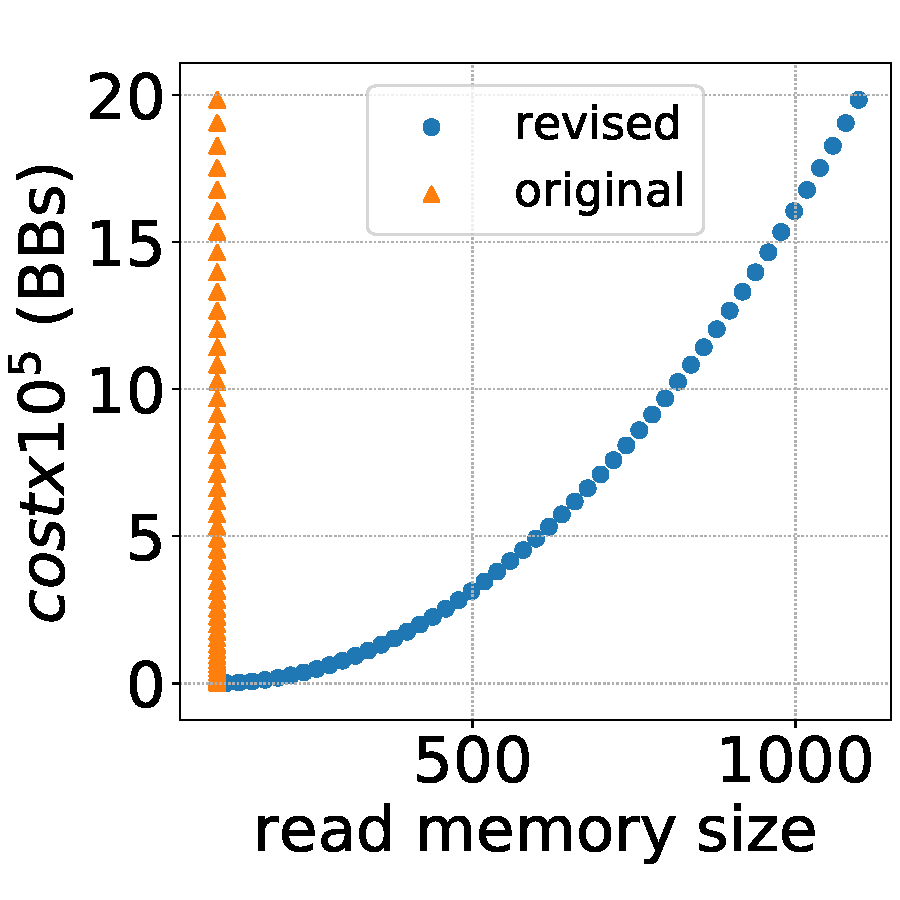
\includegraphics[width=0.32\linewidth]{figure/apache34464-line}\label{fig:bernoulli}} 
\subfloat[GCC\#27733]{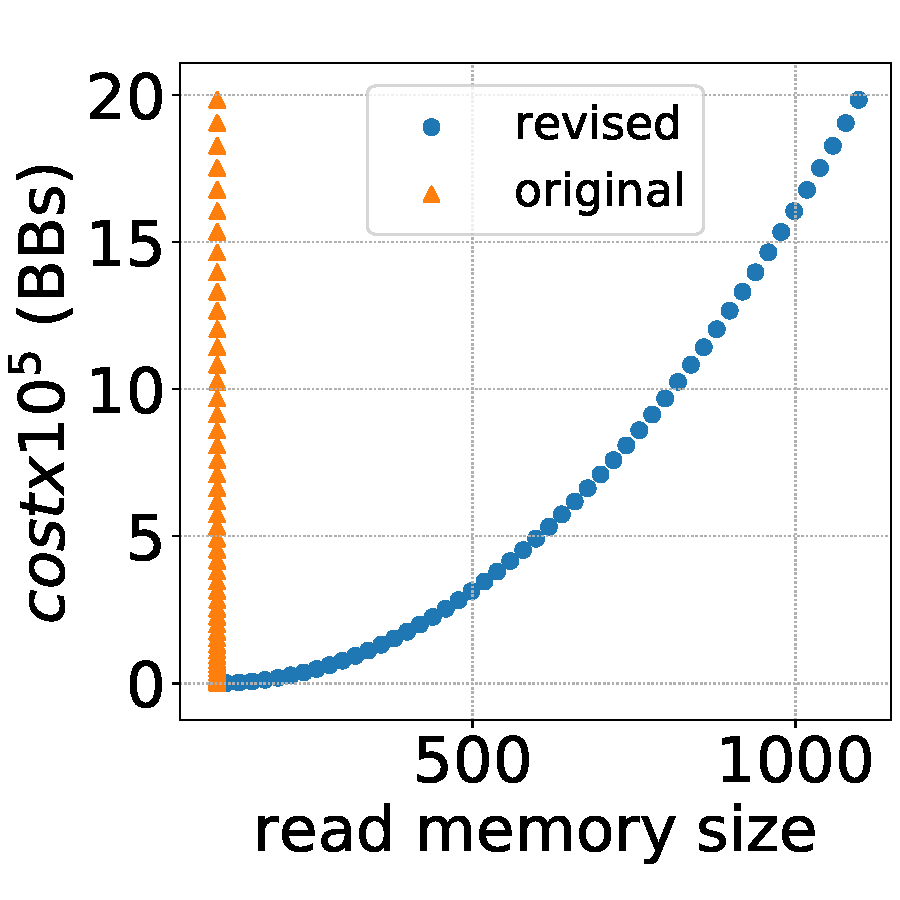
\includegraphics[width=0.32\linewidth]{figure/apache34464-line}\label{fig:jaccard}}
\subfloat[Apache\#34464]{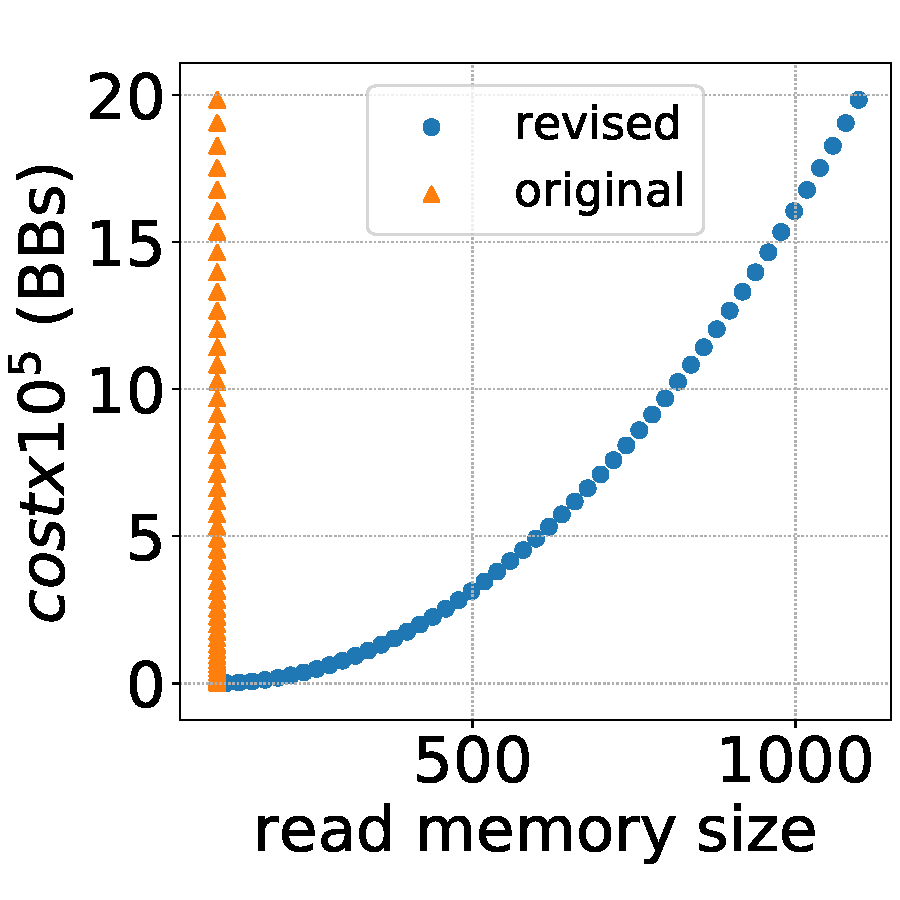
\includegraphics[width=0.32\linewidth]{figure/apache34464-line}\label{fig:apache34464-line}} \\ 
\vspace{-0.1in}
\caption{Cost function using RMS as input size.} 
\label{fig:heat} 
\end{figure*} 

Another problem for RMS is that it does not consider inputs from I/O.
Buggy code fragment for Apache\#34463 is shown 
in Figure~\ref{fig:apache34464}.
The \texttt{while} loop on line 4 searches a string \texttt{source} for a target sub-string \texttt{target}.
If the \texttt{while} loop cannot find, 
a new character from I/O function \texttt{getchar()} 
on line 6 will be appended to string \texttt{source}, 
and the loop will search string \texttt{source} again from the beginning. 
The input size for this piece of codes depend on how many characters got from \texttt{getchar()}.
Since all memory cells of string \texttt{source} are written 
firstly with characters from \texttt{getchar()} 
by this piece of codes, 
no matter how many characters we get from \texttt{getchar()}, 
the RMS value for this piece of code is constant depending 
on the size of string \texttt{target}, 
variable \texttt{sourceLen} and variable \texttt{targetLen}, 
as shown in Figure~\ref{fig:apache34464-line}. 


{\underline{\textit{Data structure size.}}}
~\citet{AlgoProf} propose to use sizes of accessed data structures, 
like linked lists or arrays, as input sizes of code constructs. 
Data structure size can provide more semantic information about analyzed codes.
However, data structure size is not a generic metric.
Special static or dynamic techniques are needed in order to identify data structures 
and figure out their sizes. 
Data structure size cannot correctly measure input size for 
a recursive function with integer value as input,
and it does not consider possible input from I/O, 
which is the same as RMS.     


{{\bf{\underline{\textit{Cost designs.}}}}
There are also a lot of metrics which can be used to measure execution cost. 
We discuss them as follows.

%\end{enumerate}
